\chapter{ILC Algorithms}
\label{ch:ILCAlg}
{\color{red} $<$Einfuerung$>$}

\newcommand{\IAgood}{30}
\newcommand{\IAbad}{50}
\newcommand{\badCondNb}{1.353$10^{16}$}

Let us imagine that we need to process the same action multiple times. 
For example, a robot manipulator must put some objects in a box with high accuracy, while the objects to put are always located in the same place. If we already have some input sequence, which solves this issue, we can use the same data for the next iteration and get the same precision. The other possibility is to ''learn'' from the previous iteration and try to enhance the exactness, while the tracking objective $r(\cdot)$ stays the same over all iterations.

More formally, we consider the system \eqref{eq:GP} over a \textit{finite time horizon} $t = 0, 1, 2, \dots, N$, $N \in \N$. As we discussed in the previous chapter, we are interested in good tracking of the signal $r(\cdot)$. At first glance, the stability concept seems to be not necessary for $N < \infty$ . Still, in this thesis, it is the requirement we presuppose on considered system. The reason is that also the discrete system over finite horizon can produce vast signals for large $N$, if the system is not stable. Especially, it means, that $A$ has at least one eigenvalue larger that one, which implies very large norm of the matrices $A^t$ for $t \gg 1$. This makes difficult the numerical calculations, since the solution of the difference equation \eqref{eq:GP} includes it. 

Moreover, for our purposes, for stabilizable systems we can assume stability without loss of generality.    
If the system is stabilizable, we can find such a matrix $F$, such that $(A - B F )$ is stable. 
We define $u(t) := - Fx(t) + \t{u}(t)$, $t = 0,1,2, \dots, N$ with a new input signal $\t u (t) \in \R^l$. Then the system \eqref{eq:GP} results in
\begin{align}
\begin{split}
x(t+1) &= (A - B F)x(t) + B \t u (t), \\
y(t)   &= (C - D F) x(t) + D\t u(t), \; t = 0, 1 ,2, \dots, N. 
\end{split}
\end{align}

We can set 
\begin{align}
\begin{array}{c c c c}
\t{A} &= (A - B F), &\t B &= B\\
\t C  & = (C - D F),&\t B & = D.
\end{array}
\end{align}
The shifted system $(\t A, \t B , \t C, \t D)$ is stable and we still can improve the input signal by considering $\t u(\cdot)$.

\begin{exam}
	\label{ex:ILC:LQR}
Let us consider the system $(A,B,C,D)$ with 
\begin{align}
\label{eq:ILC:Sys_ex1_origin}
A = \begin{pmatrix}
2 & 1 \\  4 & 3
\end{pmatrix}, B = \begin{pmatrix}
1 \\ 2
\end{pmatrix}, C = \begin{pmatrix}
0 & 1
\end{pmatrix}, D = 2.
\end{align}

This system is asymptotically stabilizable and detectable. We choose the weights $Q = 3$ and $R = 2$ and can design an LQR controller with 
\begin{align}
F =\begin{pmatrix}
1.9674  &  1.3042
\end{pmatrix} \text{ and } 
J = \begin{pmatrix}
1.8705  &  4.7321
\end{pmatrix}. 
\end{align}

To make the considered system stable we re-describe our system as
\begin{align}
\label{eq:ILC:Sys_ex1}
\begin{array}{c c c c c c c c c}
x(t+1) &=&
\begin{pmatrix}
0.0326  & -0.3042\\
0.0652  &  0.3916
\end{pmatrix}
& x(t) &+& 
\begin{pmatrix}
1 \\ 2
\end{pmatrix}
\t {u}(t)& &
\\ 
y(t)   &=& \begin{pmatrix}
	-3.9348  & -1.6084
\end{pmatrix}
& x(t)& +&
 2 \t {u} (t),& &\; t = 0, 1, 2, \dots, N. 
\end{array}
\end{align} 

We choose a piecewise constant reference $r(\cdot)$  and set $N = \IAgood$. 

With controller based on separation principle, we get the tracking illustrated in  Figure \ref{img:ILC:LQR_control}.
\begin{figure}[ht]
	\centering
	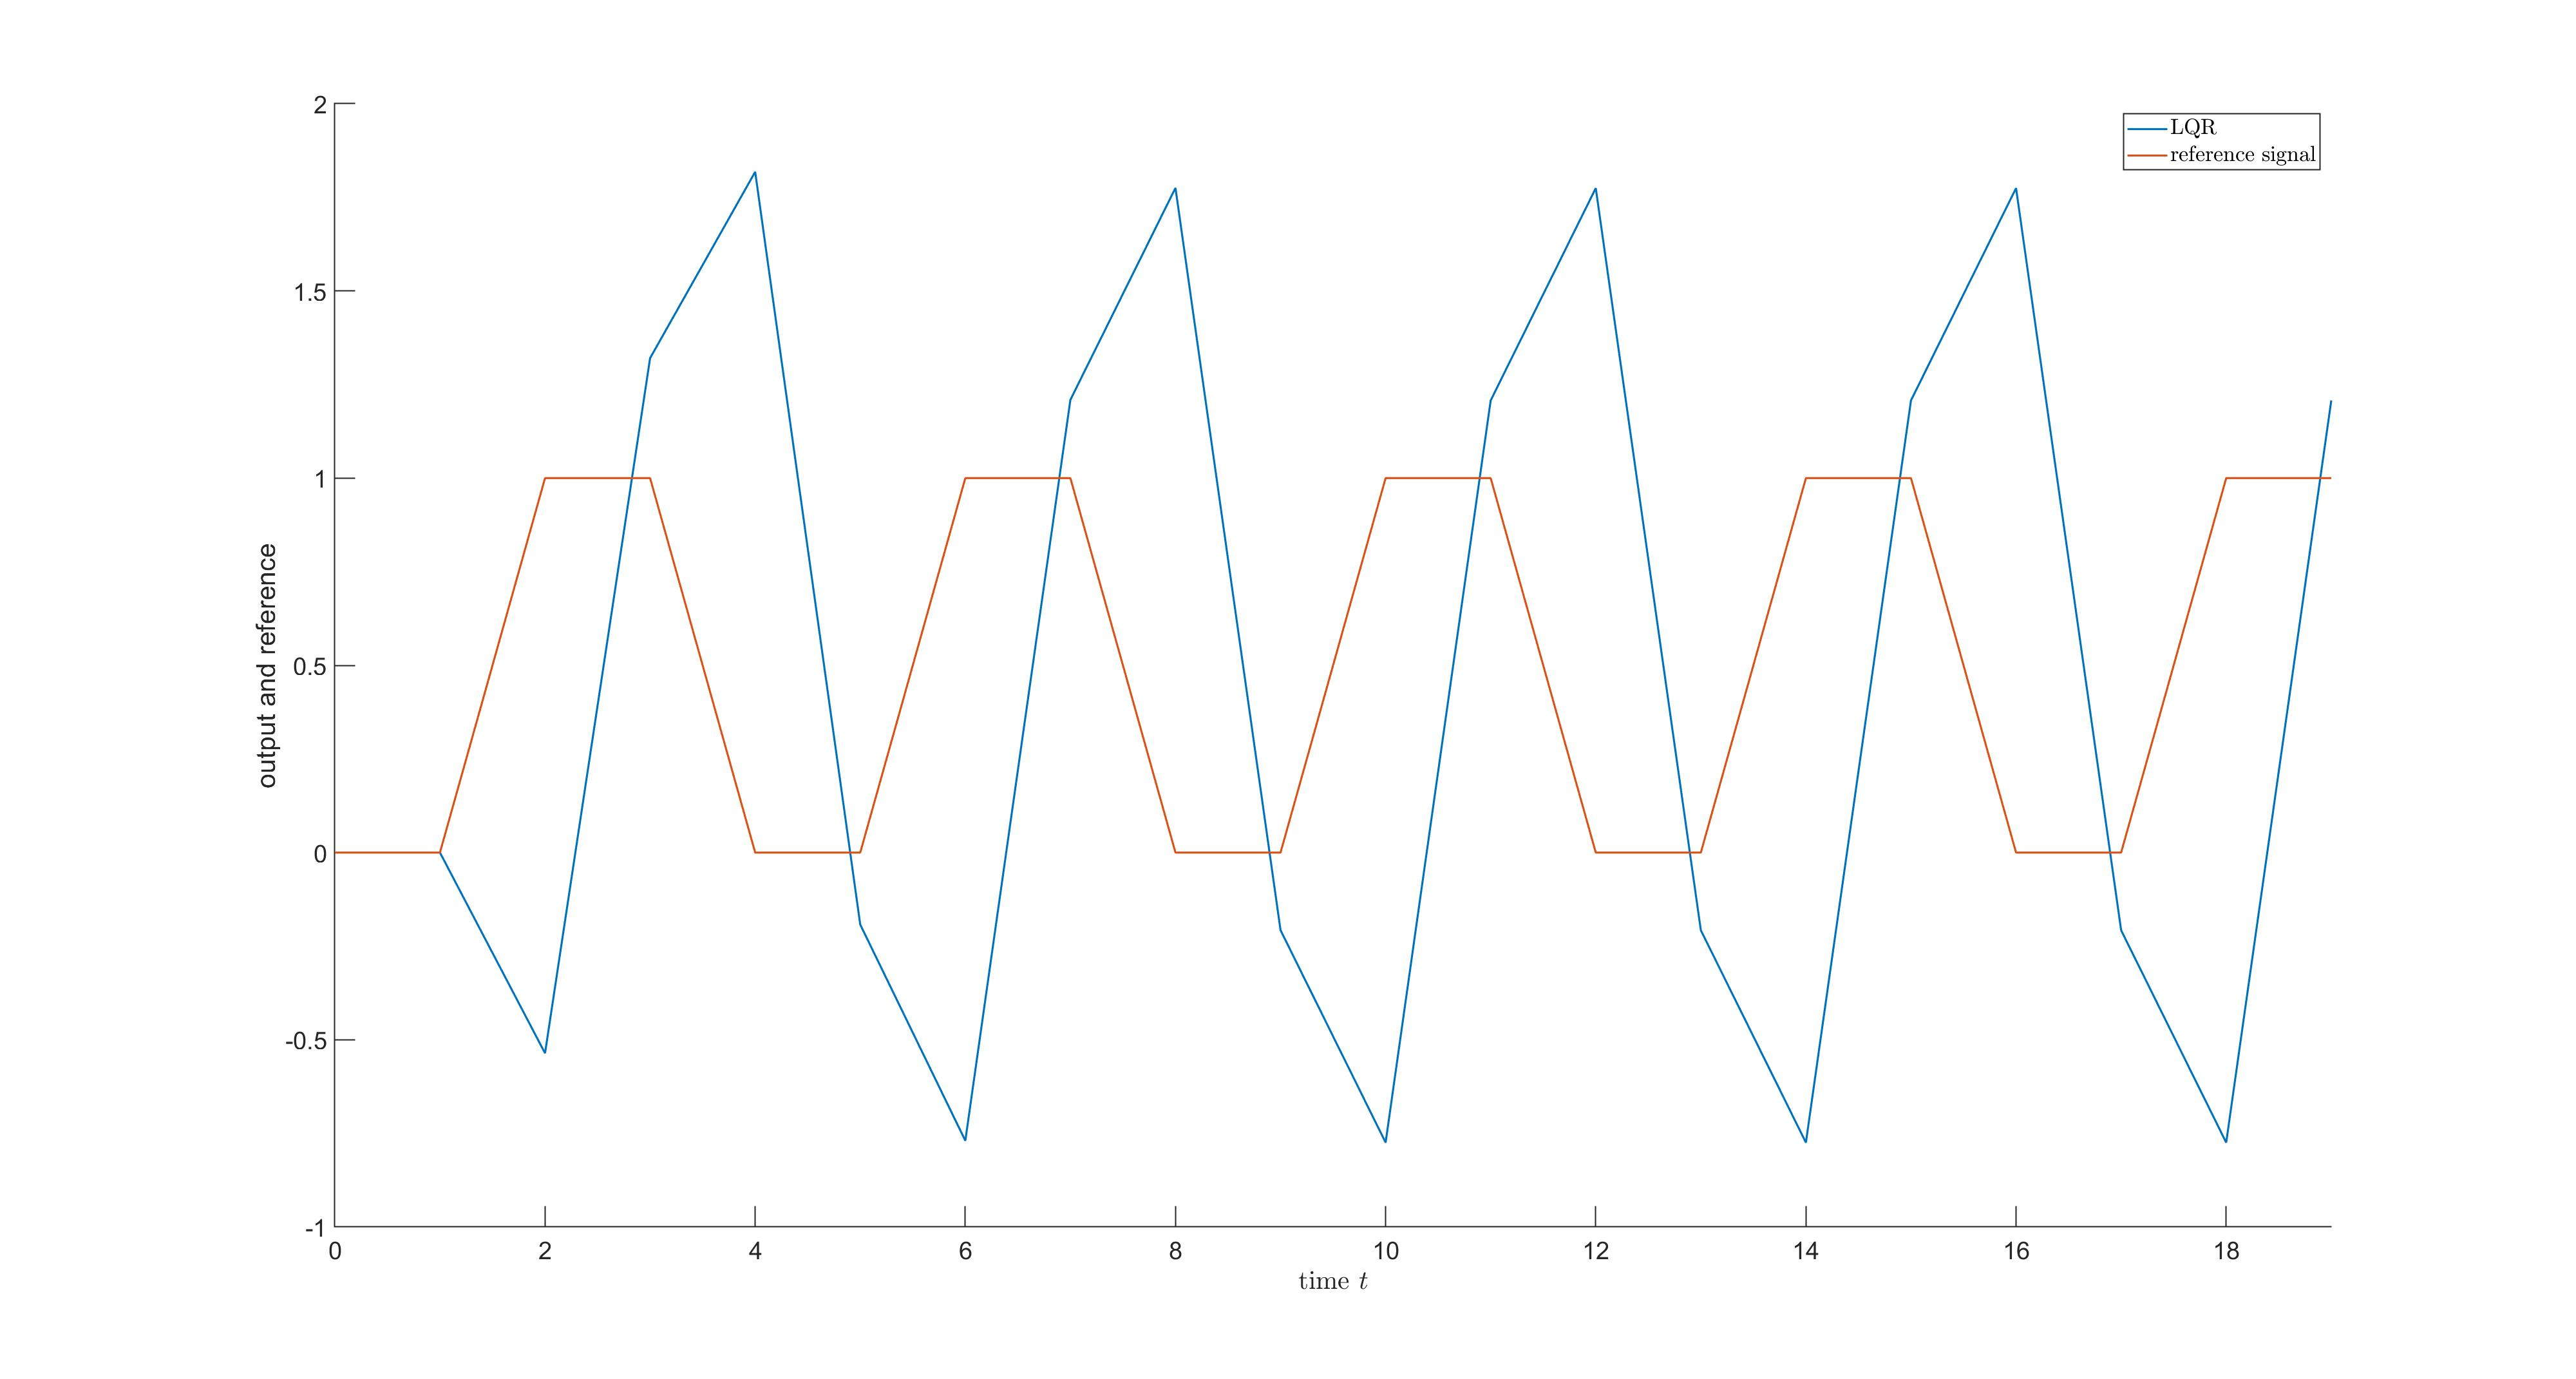
\includegraphics[width=\textwidth]{fig/Ex1_LQR.jpg}
	\caption{Tracking with LQR controller for system \eqref{eq:ILC:Sys_ex1}}
	\label{img:ILC:LQR_control}
\end{figure}
\end{exam}



As one can see, the tracking in Example \ref{ex:ILC:LQR} is not perfect. However, we can extract a bunch of information from this controlled system. For example, we get the input and output sequences 
\begin{align}
&\{u(0), \, u(1), \,  u(2) \, \dots , \, u(N)\} \subset \R^l \label{eq:ILC:u_seq}, \\
&\{y(0), \, y(1), \, y(2) , \, \dots , \, y(N)\}\subset \R^m.\label{eq:ILC:y_seq}
\end{align}
On the finite time horizon of interest the behavior of system is described by the finite input and output sequences. It seems to be an advantage. 

If we put the signals we got from simulation together, we get a large, but finite dimensional vector. That means, the standard tools from linear algebra can be applied. 

As a matter of fact, we can express our whole simulated system as a linear equation. We call such vectors \textit{supervectors}, and the whole system is said to be \textit{lifted}. This notation can describe the whole system dynamic in a compact form, and is a useful tool for ILC algorithms. 

\section{Supervector description} 

\begin{defi}
	Let $\{s(0), s(1), s(2), \dots s(N)\} \subset \R^{d}$ be a finite sequence. Then the supervector corresponding to this sequence is denoted by $s$ and is defined as 
\begin{align}
s: = \begin{pmatrix}
s(0) \\ s(1) \\ s(2) \\ \vdots \\ s(N)
\end{pmatrix}.
\end{align}
\end{defi}

In this way we define the supervectors $u \in \R^{l(N+1)} $ and $e$, $y$, $r \in \R^{m(N+1)}$. 
Analogously, we determine supervectors $r\in \R^{m(N+1)}$ and $e\in \R^{m(N+1)}$. 

For system \eqref{eq:GP} the relation between $u$ and $y$, and the error $e$ can be written in a linear matrix form 
\begin{align}
\label{eq:Gu + d}
y &= Gu + d, \\
e &= r - y.
\end{align}
The \textit{supermatrix} $G$ represents the state-space model and is given via  
\begin{align}
\label{eq:Gmatrix}
\begin{split}
G &= G(A,B,C,D) = \\
&=  \begin{pmatrix}
D & 0 & \cdots & 0 & 0 & 0 \\
CB & D & \cdots & 0 & 0 & 0\\
CAB & CB & \cdots & 0 & 0 & 0\\
\vdots & \vdots & \ddots & \vdots  & \vdots & \vdots \\
CA^{N-2} B & CA^{N-3} B &\dots &CB & D& 0\\
CA^{N-1} B & CA^{N-2} B &\dots &CAB & CB& D\\
\end{pmatrix} \in \R^{m(N+1)\times l(N+1)}.
\end{split}
\end{align}
The vector $d$ depends on the initial condition $x_0$:
\begin{align}
d = d(C,A,x_0) = \begin{pmatrix}
C x_0 \\ CA x_0 \\ CA^2 x_0 \\ \vdots \\ CA^Nx_0
\end{pmatrix} \in \R^{m(N+1)}.
\end{align}

The stability requirement for $A$ is highlighted here. In opposite to vast values for unstable matrices, we get very small terms if $N \gg 1$. Intuitive, this terms can be neglected for all $p > p^\star$ for some $1<p^\star<N$. This is usable since we can apply the sparse matrices. In the Chapter \ref{ch:Allpication} we will see, that a good estimation can be derived. 

For the system \eqref{eq:Gu + d}, the tracking problem seems to be straightforward.
If we know the reference signal $r$, we can find a perfect solution by choosing 
\begin{align}
u_\infty = G^{-1} r -d.
\end{align}

However, this choice does not look greatly credible. 
For example, if our measurements are disturbed by noise, we get the output signal
\begin{align}
y + \varepsilon w = G u_\infty + d + \varepsilon w = r + \varepsilon w \neq r,
\end{align}
for some non-zero vector $w \in \R^{m(N+1)}$ and small $\varepsilon > 0$. 

Also for uncertain models this method might be not applicable. 
If we could reformulate this idea in a more robust way, we may get a good and simple applicable algorithm, which we call the \textit{Inverse Model Algorithm.}

\section{Inverse Model Algorithms}

\begin{alg}
	\label{alg:ILC:IA}
	Let the matrix $D$ in \eqref{eq:GP} have an inverse. Then the matrix $G = G(A, B, C, D)$ is non-singular as well, and the Inverse Model Algorithm (IA) is given via input update law 
	\begin{align}
	\label{eq:errRightInv}
	\begin{split}
	u_{k+1} &= u_k + \beta G^{-1} e_k, \\
	u_0 & \in \R^{l (N+1)},
	\end{split}	
	\end{align}
	with error evolution
	\begin{align}
	\label{eq:Alg:e_k+1 = (1 - beta) e_k}
	\begin{split}
	e_{k+1} &= (1- \beta) e_{k}, \; k\geq 0, \\
	e_0 &= r -  Gu_0 -d.
	\end{split}
	\end{align}
	In particular, $(e_k)_{k\geq 0}$ converges to zero for $k \to \infty$ for any initial error $e_0 \in \R^{m(N+1)}$ if and only if 
	\begin{align*}
	0 < \beta < 2.
	\end{align*}
\end{alg}
\begin{proof}
	Firstly, the matrix $G$ has lower triangular structure, with the matrix $D$ on its diagonal. Hence, $\det(G) = \det(D)^{N+1}$, which is non-zero if and only if $D$ has full rank. 
	Taking the limit over relation \eqref{eq:Alg:e_k+1 = (1 - beta) e_k} results in
	\begin{align}
	\lim_{k \to \infty} e_{k+1} = \lim_{k \to \infty}(1- \beta) e_{k} = \lim_{k \to \infty}(1 - \beta)^k e_0.
	\end{align}
	Choosing $0<\beta < 2$ yields the proof. 
\end{proof}

For $\beta$ close to 0 or 2, we get slower convergence and better robustness. For $\beta = 1$ we get convergence in one iteration, but this choice might be non-robust \cite{ILC}, pp 149, 152-155.

We apply this algorithm on the system from Example \ref{ex:ILC:LQR} to see the algorithm performance. 

\begin{exam}
	\label{ex:ILC:badIA}
	In the system \eqref{eq:ILC:Sys_ex1} the matrix $D = 2$ is invertible, and we can apply IA. We choose as $u_0$ the input sequence of LQR controller, and $\beta = 0.1$. Convergence to 0 with tolerance $10^{-8}$ is achieved after 74 iterations.The result is illustrated in Figure \ref{img:ILC:Ex1_IA}
			
	\begin{figure}[ht]
		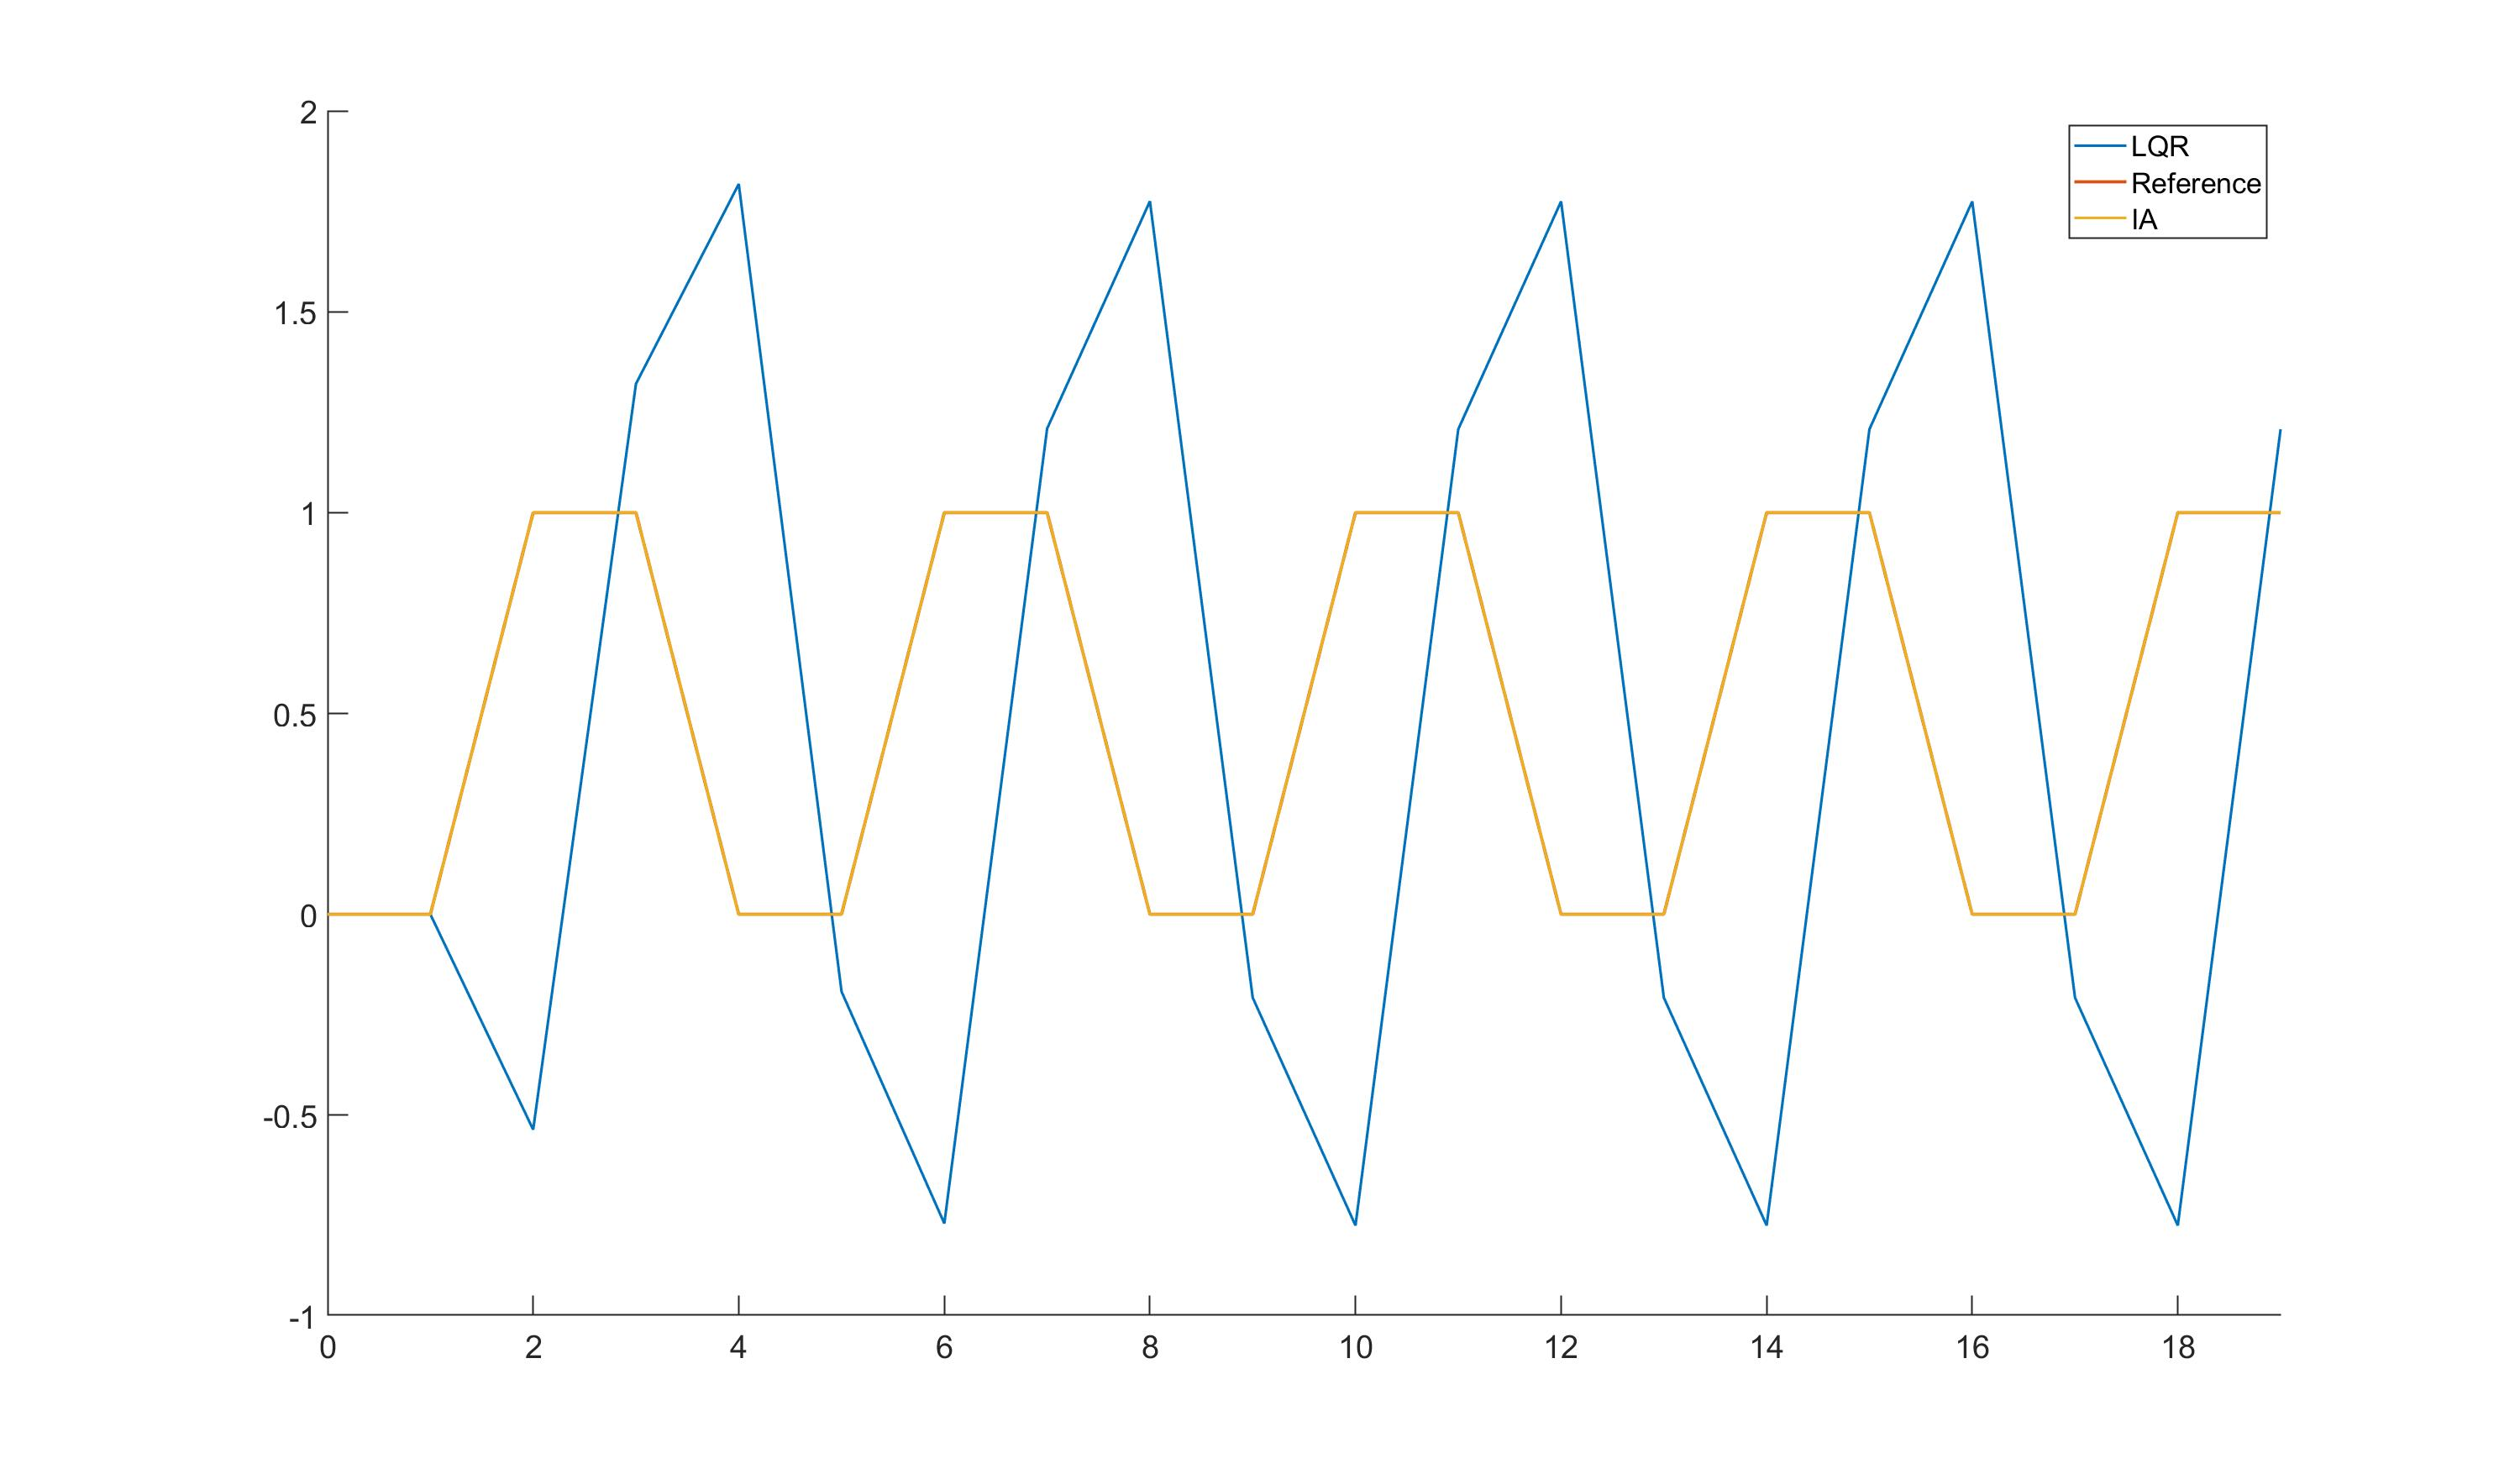
\includegraphics[width=\textwidth]{fig/Ex1_IA.jpg}
		\caption{Tracking with LQR Controller (without ILC Algorithm), and tracking with IA for the system \eqref{eq:ILC:Sys_ex1} for $N = \IAgood$}. 		\label{img:ILC:Ex1_IA}
	\end{figure}
	
	But if we try to increase the length of the time horizon $N$, for example to \IAbad steps, we can see a wrong system behavior (Figure \ref{img:ILC:Ex1_IAbad}). 
		
			\begin{figure}[ht!]
			\centering
			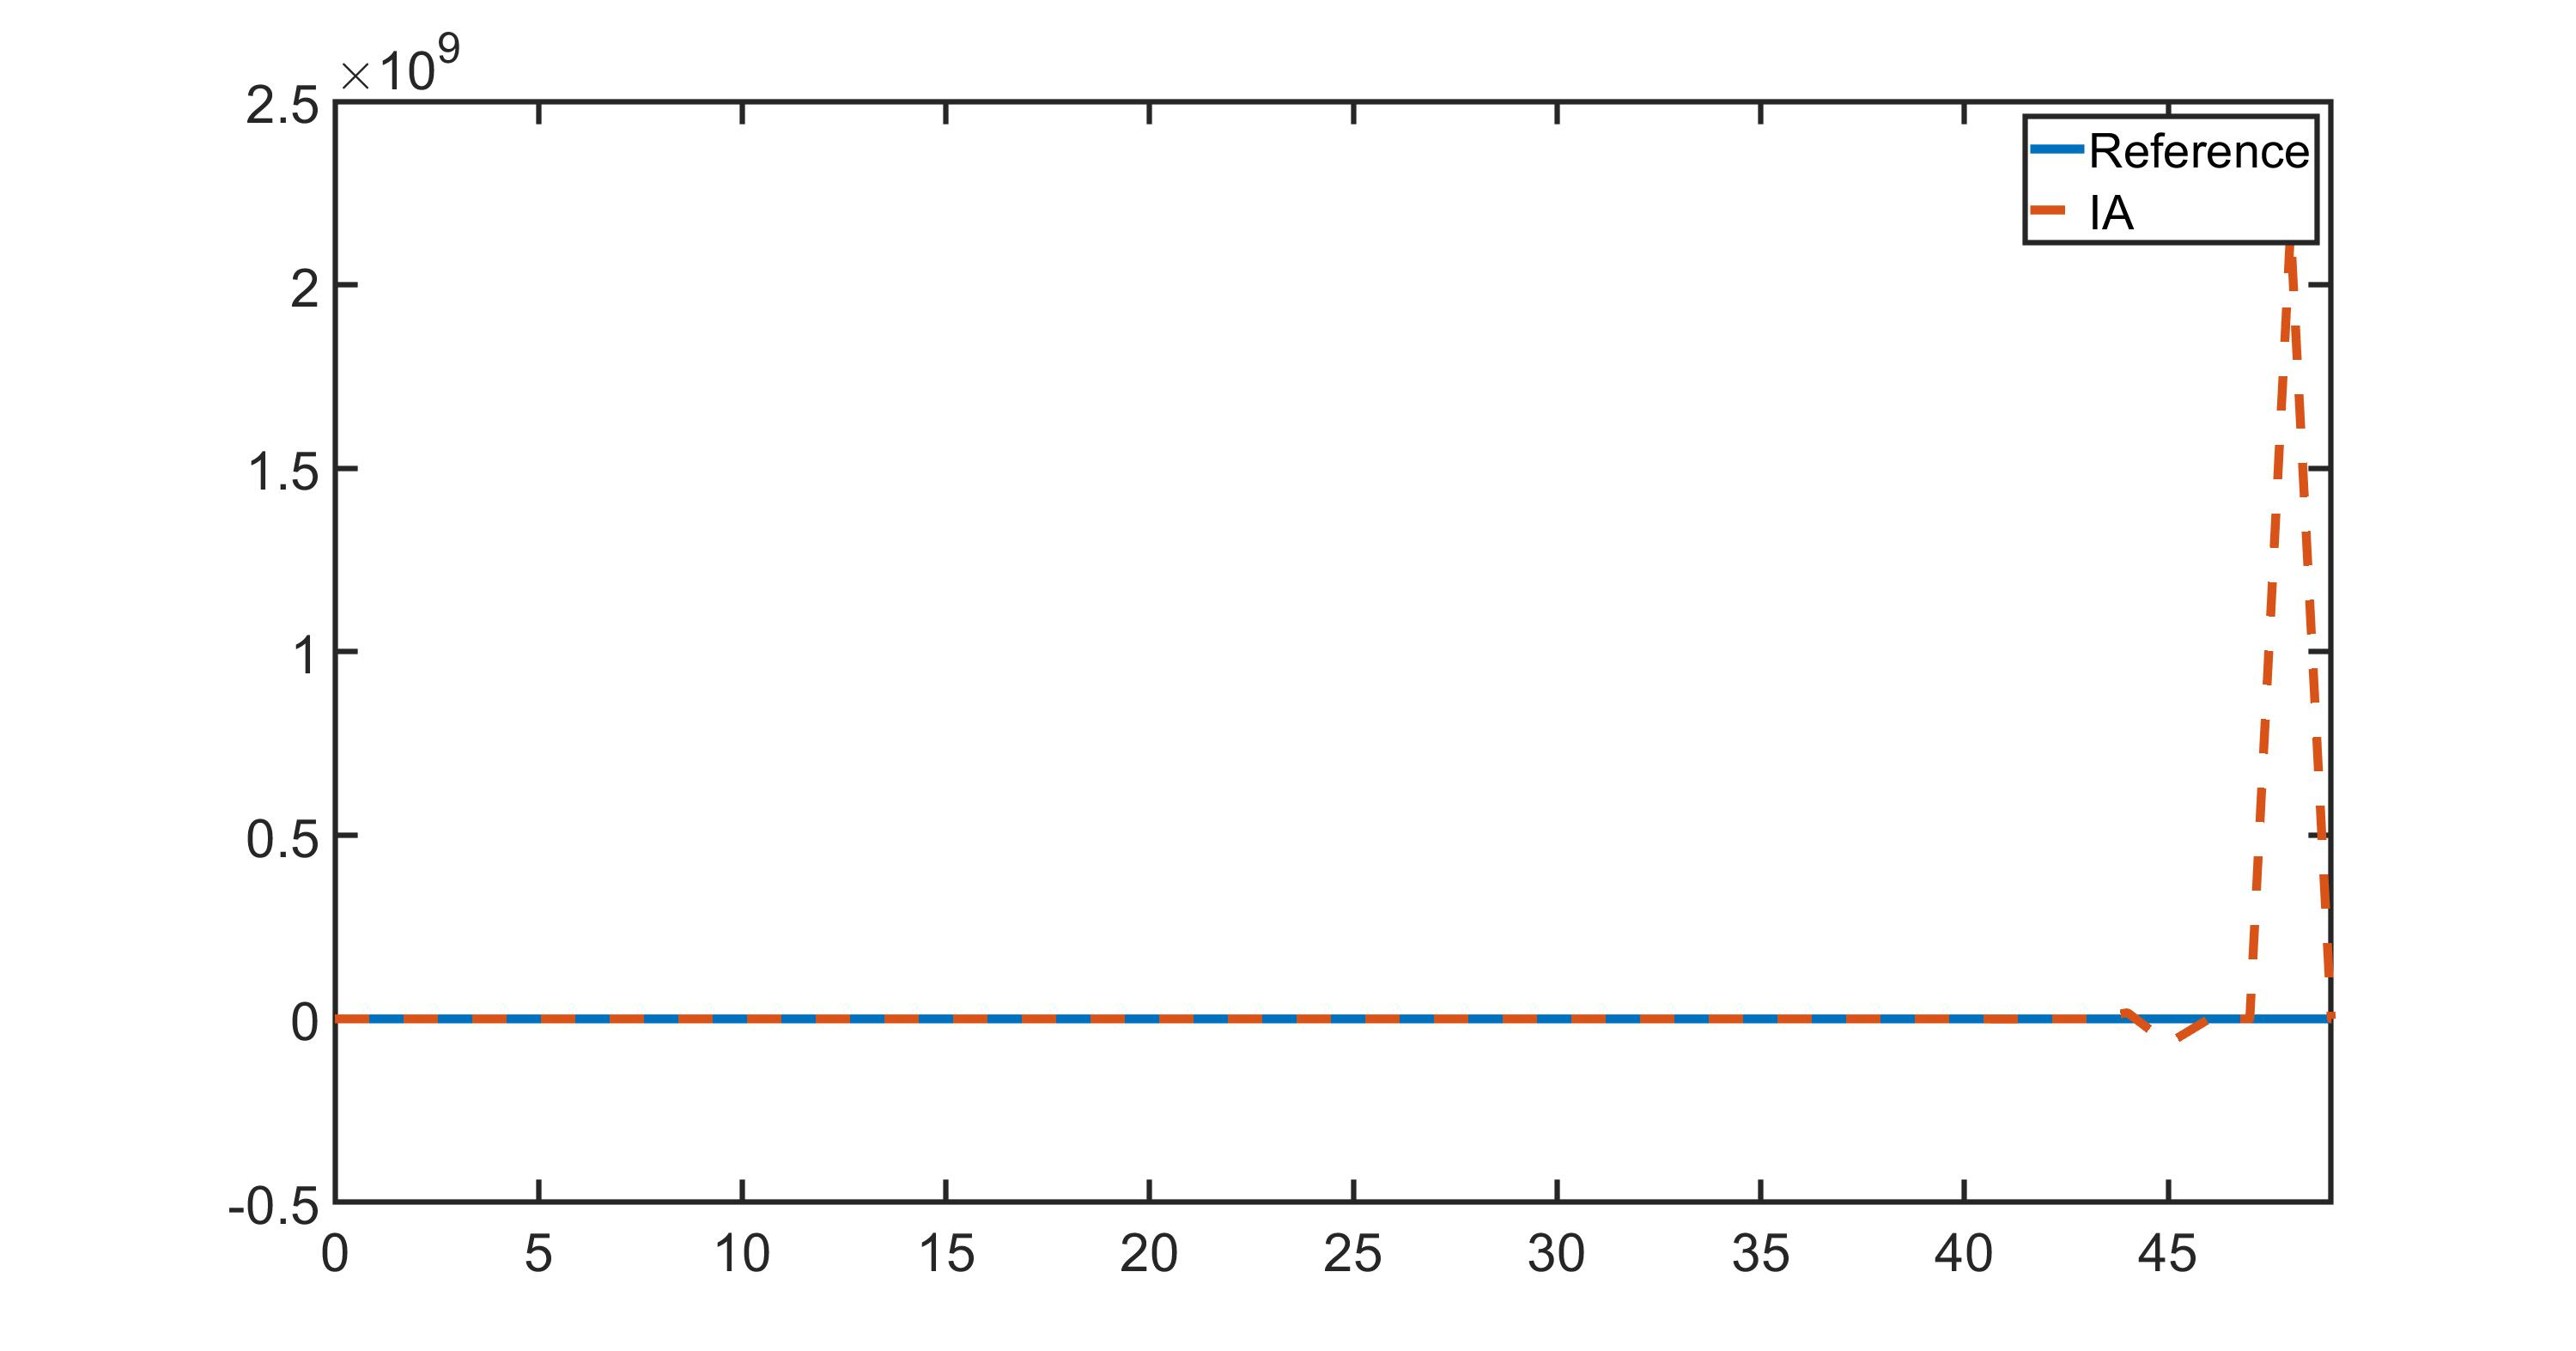
\includegraphics[width=\textwidth]{fig/Ex1_IAbad.jpg}
			\caption{Tracking with IA for the system \eqref{eq:ILC:Sys_ex1} for $N = \IAbad$}
			\label{img:ILC:Ex1_IAbad}
		\end{figure}
	
	The reason is the condition number of the matrix $G$, which equals \badCondNb. We see: even for a triangular matrix with non-zero eigenvalues, the matrix inversion can be numerically unstable.
		
		
\end{exam}

The Inverse Model Algorithm sets up very strong requirements: the matrix $G$ should be non-singular, and its condition number must be small enough we can compute a numerically stable inverse. 
We can modify this algorithm by taking the Moore-Penrose inverse. This is the so-called pseudo inverse, which is uniquely defined and can be computed for all matrices \cite{LAAG}. 

\begin{defi}
	For a matrix $G \in \R^{m(N+1) \times l(N+1)}$ a psedo inverse is defined by matrix $G^+ \in \R^{l(N+1) \times m(N+1)}$, satisfying the criteria: 
	\begin{enumerate}
		\item $G G^+ G  = G $
		\item $G^+ G G^+ = G^+$
		\item $(G G^+)^T = G G^+$
		\item $(G^+ G)^T = G^+ G$
	\end{enumerate}
\end{defi}



\begin{alg}
	\label{alg:ILC:PIA}

	The Pseudo Inverse Model Algorithm (PIA) is given via input update law 
	\begin{align}
	\label{eq:ILD:errPIA}
	\begin{split}
	u_{k+1} &= u_k + \beta G^{+} e_k, \\
	u_0 & \in \R^{l (N+1)},
	\end{split}	
	\end{align}
	with error evolution
	\begin{align}
	\begin{split}
	e_{k+1} &= (1- \beta G G^+) e_{k}, \; k\geq 0, \\
	e_0 &= r -  Gu_0 -d.
	\end{split}
	\end{align}

	Monotonic convergence to 
	\begin{align}
	\label{eq:ILC:einfPIA} 
	e_\infty  = \lim_{k\to\infty} e_k = P_{\ker[G^+]}e_0,
	\end{align} 
	is guaranteed if
	\begin{align*}
	0 <\beta < 2
	\end{align*}
	$P_{\ker[G^+]}$ denotes the positive orthogonal projection operator onto $\ker[G^+]$.
	In particular, the zero convergence is attainable, if and only if the tracking signal $r$ is feasible, that is there exists an input $\hat u$, such that $r = G \hat u$. %$e_0 \in \im [G G^\star]$. 
\end{alg}
\begin{proof}
	
	Recap the relation $(GG^+)^2 = GG^+GG^+ = GG^+$ the error evolution formula can be proven by mathematical induction: 
	
	for $k = 1$ it follows: 
	\begin{align*}
	e_1 = (I - \beta G G^+)e_0 = (I + GG^+ - GG^+ - \beta G G^+)e_0 = (I + \left[(1 - \beta) + 1\right]GG^+)e_0.
	\end{align*}
	
	For $k \in \N$  
	\begin{align*}
	e_{k+1} &= ( I - \beta G G^+)e_k = ( I - \beta G G^+) (I+  \left[(1-\beta)^{k-1} - 1\right] G G^+) e_0 = \\
	& = \left(I - \beta G G^+ + (1-\beta)^{k-1}GG^+ - GG^+ - \beta GG^+\left[(1 - \beta)^{k-1} - 1\right]GG^+\right)e_0=\\
	& = \left(I - (\beta - (1-\beta)^{k-1} + \beta\left[(1 - \beta)^{k-1} - 1\right])G G^+\right)e_0\\
	& = \left(I - \left(\beta - (1-\beta)^{k-1} + 1 + \beta(1-\beta)^{k-1} - \beta\right)GG^+\right)e_0\\
	& = (I+  \left[(1-\beta)^k - 1\right] G G^+) e_0
	\end{align*}
	
	To prove \eqref{eq:ILC:einfPIA}  recall that 
	\begin{align*}
	\R^{m(N+1)} = \im(G)\oplus \ker (G^+),
	\end{align*}
	$\oplus$ denotes here the direct sum of two vector spaces. 
	Hence $e_0$ can be written as 
	\begin{align*}
	e_0 = G w_0 + v_0,
	\end{align*}
	where $v_0 = (I - G G^+)e_0 \in \ker (G^+)$  is uniquely defined and $w_0 = G^+ e_0 \in \R^{l(N+1)}$. It follows: 
	\begin{align*}
	e_{k} = (1+ \left[(1 - \beta)^{k-1} - 1\right]GG^+)e_0 = (1-\beta)^{k-1} G w_0 + v_0.
	\end{align*}
	Then for $\beta \in (0,2)$ the error $e_k$ converges to $v_0$ for $k \to \infty$. 
\end{proof}

\begin{exam}
	\label{ex:ILC:PIA}
	We calculate a solution for \eqref{eq:ILC:Sys_ex1} with PIA, and illustrate it in Figure \ref{fig:ILC:Ex1_PIA}. 	
	This time the tracking signal and system output fit well despite the large condition number. However, a deviation can be observed at the beginning, which causes the bad invertability of the matrix $G$. 
	  
	\begin{figure}[ht!]
		\centering
		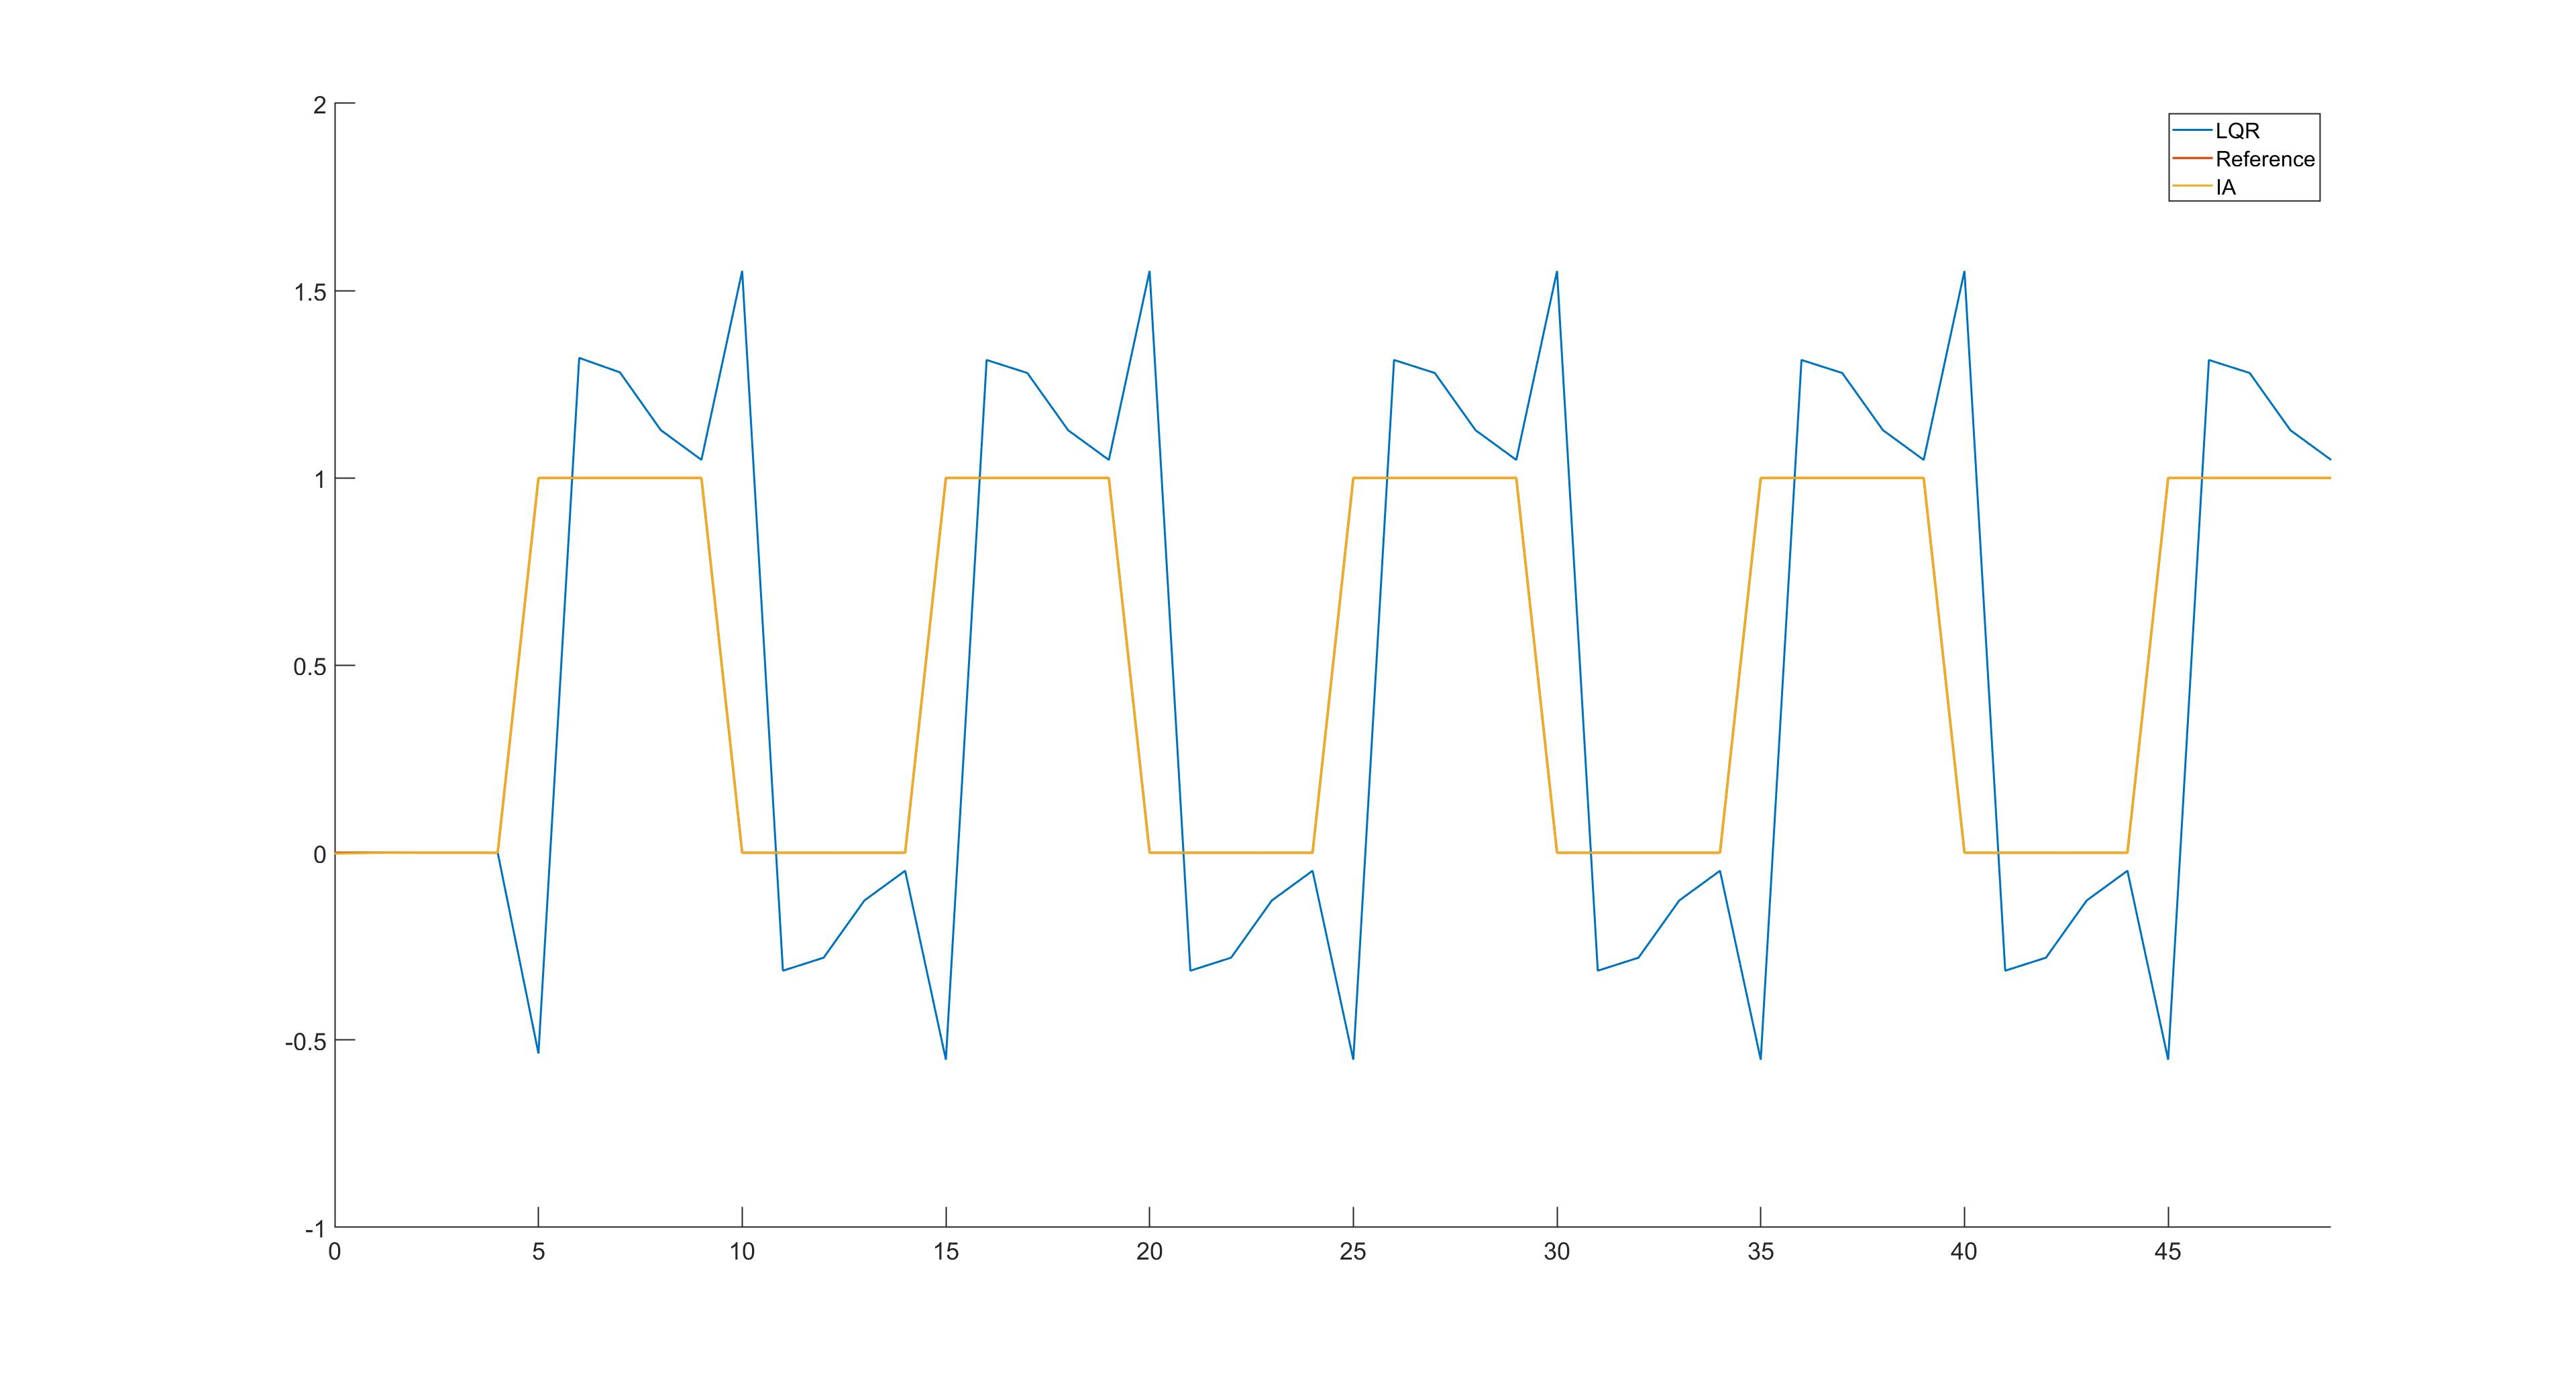
\includegraphics[width=\textwidth]{fig/Ex1_PIA.jpg}
		\caption{Reference signal tracking with LQR and PIA for the sysytem \eqref{eq:ILC:Sys_ex1} for $N = \IAbad$ }
		\label{fig:ILC:Ex1_PIA}
	\end{figure}
\end{exam}


We can replace the use of pseudo inverse by taking a left or right inverse, if it exists. 
However, it  only makes sense if the calculating afford or numerical stability are better for left or right inverse calculation. 

The pseudo inverse has its advantage to equal the right/left inverse, if it exists. Moreover, for right/left inverse we need to restrict the rank requirements, as it exists not for every matrix. 
The algorithm in this formulation can be applied for any matrix $G$. 

The Algorithm \ref{alg:ILC:IA} is a special case of PIA. However, numerically the use of inverse matrix might be more desirable since the calculation effort, if the condition number is not large. 

(Pseudo) Inverse Algorithm belongs to the class of so-called Unit Memory Algorithms -- these are the algorithms we assume to  ''remember'' the last trial. 

\section{Unit Memory Algorithm}

We are interested in  the processes, which are executed repetitively. Let $k = 0, \, 1, \, 2, \, \dots $ be the number of completed iterations. Then we get a system 
\begin{align}
\label{eq:unitMemory}
\begin{split}
y_{k} &= G u_k + d,  \\ %& &\text{ (The Input Update Rule)} 
e_k &= r - y_k, 
\end{split}
\end{align}
$u_{0} \in \R^{l(N+1)},  \; k =0, \,  1, \, 2, \dots $.
%This is again a discrete-time system, with time increment $k$. 

To achieve a good tracking at trial $k$ we need to ensure that the norm $||e_k||$ is small. 
The tracking behavior improves for consecutive iterations if the sequence $||e_k||$ is monotonically decreasing, i.e., 
\begin{align}
||e_{k+1} || < ||e_k|| \text{ for all } k \geq 0.
\end{align}
Note that in this case the sequence $||e_k||$ is guaranteed to converge. If the sequence even converges to zero we say that perfect tracking is achieved asymptotically.


We have already seen, that it is not always possible to achieve zero convergence. In Algorithm \ref{alg:ILC:PIA} the perfect tracking is possible, if the reference signal $r$ is feasible -- that is, there exists an input signal $u_\infty$, such that $r = G u_\infty + d$. In common the convergence properties can also depend on the choice $u_0$.

%the monotonic convergence to some $e_\infty \in \R^{m(N+1)}$ is desirable :
%\begin{align}
%\lim_{k \to \infty} e_k = e_\infty, \text{ and } ||e_{k+1} || \leq ||e_k|| \text{ for all } k \geq 0.
%\end{align}

%First we try to formulate an iteration law for the input signal, and calculate then the error sequence as 
%\begin{align}
%e_k = r - y_k = r - G u_k - d, k \geq 0.
%\end{align}

We assume linear dependency of $u_{k+1}$ upon $u_k$ and $e_k$ for $k \geq 0$, and define the following algorithm using feedback control. 
\begin{alg}
	\label{alg: unitMemory}
	The Unit Memory Algorithm is given via input update law 
	\begin{align}
	\label{eq:clPlant}
	\begin{split}
	u_{k+1} &= u_k + K e_k, \\
	& u_0 \in \R^{l (N+1)}.
	\end{split}
	\end{align}	 
	The error dynamic is then given via
	\begin{align}
	e _{k+1} &= (I - G K) e_{k}, \; k \geq 0,\\
	e_0 &= r -  Gu_0 -d.
	\end{align}
%	since 
%	\begin{align}
%	\begin{split}
%	e_{k+1} &=  r - y_{k+1} = r - G u_{k+1} - d =\\
%	&= r - Gu_k - G Ke_k - d = e_k - G Ke_k, \; k\geq0.
%	\end{split}
%	\end{align}
	$K \in \R^{l(N+1) \times m(N+1)}$ is called \textbf{learning matrix}. 
\end{alg}

To ensure the stability of the algorithm, it is enough to consider the iteration process 
\begin{align}
\label{eq:e_k}
e_{k+1} = (I - G K) e_k = (I - G K)^k e_0  : =  L^k e_{0}, \; k \geq 0.
\end{align}

That it is a discrete time dynamical system over $k$. We can reformulate our goal as follows: find some matrix $K \in \R^{l(N+1) \times m (N+1)}$, which renders \eqref{eq:e_k} stable. %In other words, we are looking for a stabilizing controller $K$. 

If we rewrite our system as
\begin{align}
\label{eq:ILC:e_kPlant}
\begin{pmatrix}
e_{k+1} \\ e_k
\end{pmatrix} = 
\left(
\begin{array}{c|c}
I & -G \\\hline I & 0
\end{array}\right) \begin{pmatrix}
e_k \\ v_k 
\end{pmatrix},
\end{align}
our problem reduces to finding a stabilizing controller $K$  with 
\begin{align}
v_k = K e_k.
\end{align} 

We know how to work with such systems -- for example, LQR controller provides a good solution. This is a reliable method, but since the matrix $G$ can have large dimension, it also can be costly. Often we can achieve good results with much more simple methods. For example, we can reduce the number of parameters to be chosen. 

In the Algorithms \ref{alg:ILC:IA} and \ref{alg:ILC:PIA} we chose a fixed matrix $K_0$ as the (pseudo) inverse of $G$, and left the parameter $\beta$ to decide on. So, we reduced the number of degrees of freedom to 1, and still get satisfying results.


However, as we have seen in Example \ref{ex:ILC:badIA}, the calculation of the  inverse matrix is not the most reliable method. The pseudo inverse refers better results, but is also much more expensive. 

An algorithm, which does not require the model inversion, might be here of use. 

	 \section{Gradient Algorithms}
We want a new algorithm to render monotonic convergence. 
The direct calculation provides 
\begin{align}
\label{eq:monConv}
||e_{k+1}|| < ||e_k|| \text{ for all } k >0,
\end{align}

in some norm $|| \cdot || $ in $\R^{m(N+1)}$. 

We chose positive definite weighting matrices $Q(t)$ and $R(t)$, $t = 0, 1, 2, \dots ,N$, and define the scalar products
\begin{align}
\label{eq:SkPrQR}
\langle y,z\rangle_Q = \sum_{t = 0}^N y(t)^TQ(t)z(t), \; \langle u,v\rangle_R = \sum_{t = 0}^N u(t)^T R(t) v(t),
\end{align}
with $y(t), z(t) \in \R^{m}$, $u(t), v(t) \in \R^l$ for $t = 0,1,2, \dots, N$.

We denote with $||\cdot||_Q$ and $||\cdot||_R$ the associated norms, and set
\begin{align*}
G^\star &= R^{-1} G^T Q \text{ for all } G \in \R^{m(N+1)\times l(N+1)},\\
K^\star &= Q^{-1} K^T R \text{ for all } K \in \R^{l(N+1)\times m(N+1)},
\end{align*}
where 
\begin{align}
Q := \diag(Q(0), Q(1), Q(2) ,\dots, Q(N)) \text{ and } R:= \diag(R(0), R(1), R(2), \dots, R(N)).
\end{align}
%In the same way, we can define 
%\begin{align}
%L^\star &= Q^{-1} L^T Q \text{ for all } L \in \R^{m(N+1)\times m(N+1)} \text{ and }\\
%M^\star &= R^{-1} M^T R \text{ for all } M \in \R^{l(N+1)\times l(N+1)}.
%\end{align}

Recall, that for $R = I$ and $Q = I$ the matrices $G^\star$ and $K^\star$ are just the conjugate transpose. The notation from above can be seen as conjugate transpose in the vector space with scalar products \eqref{eq:SkPrQR}.

Applying the weighted norms on \eqref{eq:monConv} provides
\begin{align}
\begin{split}
||e_{k+1} ||_Q^2 &= ||e_k - G K e_k||_Q^2 = ||e_k||_Q - 2\langle e_k , G K e_k \rangle_Q + ||G K e_k||_Q^2 \\ 
&< ||e_k||_Q^2, \text{ if } ||GK e_k||_Q^2 < 2 \langle e_k, GK e_k\rangle_Q. 
\end{split}
\end{align}

The last inequality is equivalent to 
\begin{align}
e_k^T K^T G^T Q GK e_k < 2 e_k^T Q GK e_k.
\end{align}

If we set $K = \beta G^{\star}$ this is implicated by 
\begin{align}
\label{eq:ILC:SDA_Herleitung}
\beta^2 (G G^{\star})^T Q (G G^{\star}) \prec \beta Q G G^{\star} + \beta (Q G G^{\star})^T.
\end{align}

Since the matrix $Q$ is positive definite, we can find a positive definite 	 matrix $Q^{1/2}$, such that $Q = Q^{1/2}Q^{1/2}$. 

We write $Q^{-1/2}$ for $\left(Q^{1/2}\right)^{-1}$, and define a matrix 
\begin{align}
H :=  Q^{1/2} G G^\star Q^{-1/2}. 
\end{align}
The matrix $H$ has the same eigenvalues as $G G^{\star}$, as for its characteristic polynomial holds 
\begin{align}
\begin{split}
\det (I - \lambda H) &= \det \left(I - \lambda Q^{1/2} G G^\star Q^{-1/2}\right) \\
&= \det\left(Q^{1/2}\right)\det\left(I - \lambda G G^\star\right) \det\left(Q^{1/2}\right)^{-1} \\
&= \det\left(I - G G^\star\right) \text{ for any } \lambda \in \R. 
\end{split}
\end{align}

We rewrite \eqref{eq:ILC:SDA_Herleitung} as 
\begin{align}
\beta^2 H^T H \prec \beta (H + H^T). 
\end{align}

This relation is fulfilled if 
\begin{align}
0 < \beta < \frac{2}{\lama(H)}. 
\end{align}


This deliberation inspires the \textit{Steepest Descent Algorithm}. 

\subsection{Steepest Descent Algorithm}
\begin{alg}
	\label{alg:SDA}
	The Steepest Descent Algorithm is characterized by choosing $K = \beta G^\star$, where $\beta>0$ is a real scalar gain. The input update law is given via 
	\begin{align}
	\label{eq:errSDA}
	\begin{split}
	u_{k+1} &= u_k + \beta G^\star e_k,\\
	u_0 &\in \R^{l (N+1)}, 
	\end{split}
	\end{align}
	and error evolution results in 
	\begin{align}
	e_{k+1} &= (I- \beta G G^\star) e_{k}, \; k\geq 0.
	\end{align}
	Monotonic convergence to 
	\begin{align}
	\label{eq:SDAErrLim} 
	e_\infty  = \lim_{k\to\infty} e_k = P_{\ker[G^\star]}e_0,
	\end{align} 
	is guaranteed if
	\begin{align*}
	0 <\beta < \frac{2}{\lama(H)}.
	\end{align*}
	Convergence to zero is assured in the case that $e_0 \in \im [G G^\star]$ holds.
\end{alg} 
\begin{proof}

To prove the statement remember that, as $GG^\star$ is a symmetric matrix, we can find unique vectors 
$e_{\im} \in \im(G G^\star)$, $e_{\ker} \in \ker(G G^\star)$, such that 
\begin{align}
e_0 = e_{\im} + e_{\ker}.
\end{align}


Substituting $e_0$ in error evolution by this expression we get  
\begin{align}
e_{k+1} = (I - \beta G G^\star) e_k = (I - \beta G G^\star)^k e_{\im} + e_{\ker}.
\end{align}

For convergence to $e_{\ker}$ it is enough  to show that $\lama(I - \beta G G^\star) < 1$: as $(I - \beta G G^\star)$ is a symmetric matrix, the convergence is guaranteed if and only if all the eigenvalues of $(I - \beta G G^\star)$ are less than 1 in its absolute value. 

If $\lama(I - \beta G G^\star) = 0$, then $(I - \beta G G^\star) = 0$  and convergence follows trivially. 

Let $0 \neq \mu \in \C$ be an eigenvalue of the matrix $(I - \beta G G^{\star})$. Then there exists some $0 \neq v \in \R^{l (N+1)}$, such that 
\begin{align}
	(I -\beta G G^{\star})v = \mu v \Rightarrow G G^{\star} v = \frac{1 - \mu}{\beta}v. 
\end{align}

Since our choice of $\beta$, the inequality \eqref{eq:ILC:SDA_Herleitung} holds and implies 
\begin{align}
\beta^2 v^T (G G^\star)^T Q (G G^\star) v < 2\beta v^T(Q G G^\star)v 
\Rightarrow (1 - \mu)^2 ||v||_Q < 2 (1 - \mu) ||v||_Q. 
\end{align}

This is the case if and only if the absolute value of $(1 - \mu)$ is less than 2: 
\begin{align}
|1 - \mu| < 2. 
\end{align}

It concludes $|\mu|<1$ and proves the convergence. 
\end{proof}



An interesting observation is, that via this algorithms got input signal $u_\infty$ is the unique solution of the (minimum norm) optimization problem 
\begin{align}
u_\infty = \arg \min_{u \in \R^l(N+1)} \{|| u - u_0||_R^2: \text{ subject to } r = Gu + d\}.
\end{align}
One consequence is that the choice of $u_0$ has more significance than the simple intuition. A good choice will influence convergence rates beneficially. More generally, the limit $u_\infty$ is the closest input to $u_0$ in the norm, and since choosing $u_0 = 0$ leads to minimum energy solution $u_\infty$ \cite{ILC} p. 168. 

\textbf{Choice of the Weighting Matrices}

The choice of the weighting matrices $Q$ and $R$ provides us additional degrees of freedom. 
Using them we can impact the behavior of the algorithm. For example, with the choice of the matrix $Q$ we can weight some elements of inputs and outputs signals, depending on their importance in measuring accuracies and convergence rates, or accent the relative importance of different time intervals in measuring tracking accuracy and required convergence rates. For rapidly convergence in the initial parts of the time interval, we can set $Q(t) = \varepsilon^{2t}\tilde{Q}$ with some time independent $\tilde{Q}$ and $\varepsilon \in (0,1)$. 

The choice of $R(\cdot)$ may arise out of the real need to converge to a minimum input energy solution. 
Again, using the $\varepsilon$-weighed $R(t) = \varepsilon^{2t}\tilde{R}$ with some fixed $\tilde{R}$, we can accent the input signals at some times $0\leq t_1 \leq t \leq t_2 \leq N$. This can be used if we want to limit the control action at some time intervals, or if we need to reflect the physical units used. 

\begin{exam}
	In the Example \ref{ex:ILC:PIA} we could not achieve perfect tracking at first trials. 
	We can improve it by using the SDA, if we choose adequate weight $Q$. 
	
	With choice 
	\begin{align}
	Q =  \diag \begin{pmatrix}
		10^{-2} & 1 & 1 & 1 & 10^{-2} & \dots &10^{-2}
	\end{pmatrix}.
	\end{align}
	we speed up the convergence at the second, third and fourth time step. 
	
	The result is illustrated in Figure \ref{img:ILC:Ex1_SDA}. 

	\begin{figure}[ht]
		\centering
	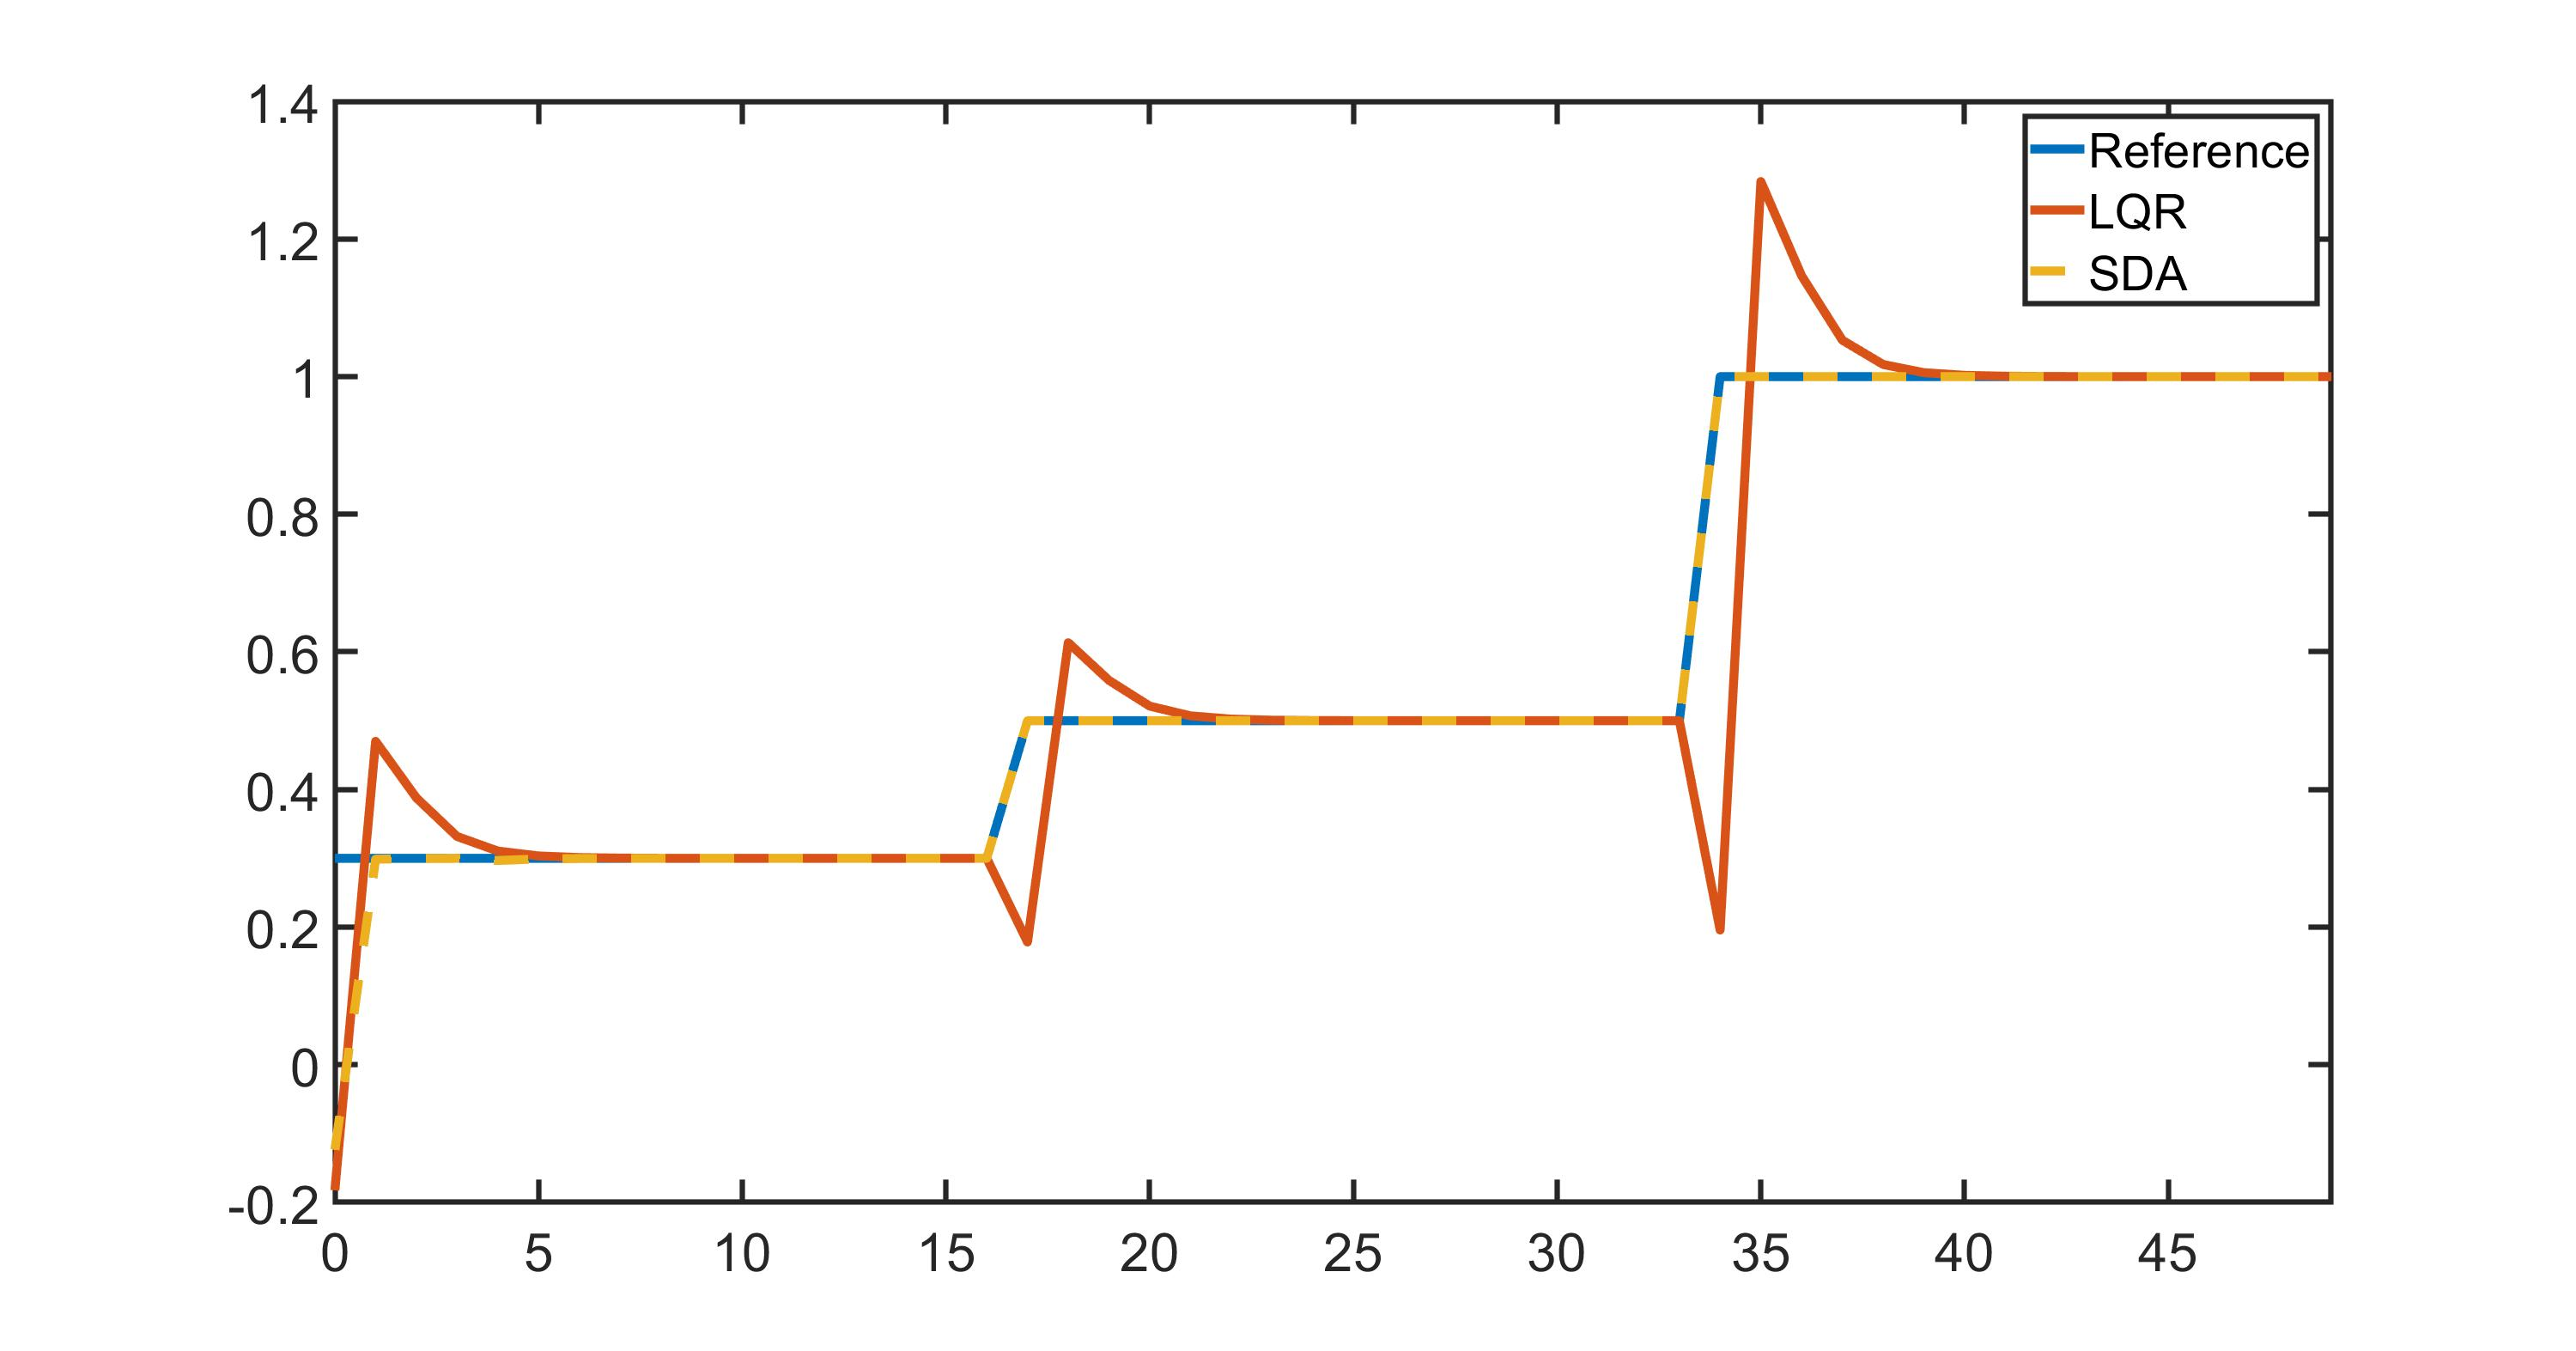
\includegraphics[width=\textwidth]{fig/Ex1_SDA.jpg}
	\caption{Reference signal tracking with LQR and SDA for the system \eqref{eq:ILC:Sys_ex1}}
	\label{img:ILC:Ex1_SDA}
\end{figure}

By choosing the weight $R$ we can regulate the control action. As we limit the possible input signals, it also leads to a rapid convergence. For example, for $R = I$ we need 8124 iterations, while with 
\begin{align}
R = \diag \begin{pmatrix}
1& 1 & 1 & 1 & 0.1 & \dots & 0.1
\end{pmatrix}
\end{align}
only 2569 trials are required. 

\end{exam}


\subsection{Suppression of eigenvalues} 

In the previous algorithms we assumed the learning matrix $K$ to be constant for all iterations.
We can presume another controller structure and set variable $K_k$ for $k\geq 0$. 

The simplest modification way is to set an iteration varying gain $\beta$ for each step: $K_k = \beta_k K_0$, $k\geq 0$ for a fixed matrix $K_0$. 

Let us consider the eigenvalues of the matrix $GG^\star$ and choose the gains $\beta_k$, $k \geq 0$ according to them. 

\begin{theo}
	Assume, that the matrix $GG^\star$ has $q+1$ non-zero ordered eigenvalues $\lambda_0, \lambda_1, \dots ,  \lambda_q$. Set $\beta_k = \frac{1}{\lambda_k}$ for $k = 0, 1, \dots, \, q$ and consider the update law
	\begin{align}
	\label{eq:cl_var0}
	\begin{split}
	u_{k+1} &= u_k + \beta_k G^\star e_k, \\
	e _{k+1} &= (I - \beta_{k+1}  GG^\star) e_{k}  = \prod_{l = 0}^{k+1} (I - \beta_{l}  GG^\star) e_0, \; k\geq 0,\\
	u_0 &\in \R^{l (N+1)}.
	\end{split}
	\end{align}
	Then the error sequence $(e_k)_{k\geq 0}$ converges in a finite number of iterations.     
\end{theo}
\begin{proof} 
	Set $\t{N} := m(N+1) - 1$. With spectral theorem, there exists a basis of the eigenvectors $\{v_0, v_1, \dots, v_{\t N}\}$ with corresponding eigenvalues $\lambda_0, \lambda_1, \dots, \lambda_q, 0, \dots 0$. 
	Then we can write $e_0$ as 
	\begin{align}
	e_0 = \sum_{p = 0}^{\t N} \gamma_p v_p
	\end{align}
	with uniquely defined $\gamma_p \in \R$, $p = 0, 1, \dots, \t N$. 
	
	For $k \in \N$ it follows 
	\begin{align}
	e_k = \left(\prod_{j=0}^k(I - \beta_j G G^\star)\right)e_0 = \sum_{p = 0}^{\t N} \gamma_p \left(\prod_{j=0}^k (I - \beta_j \lambda_p I)\right)v_p.
	\end{align}
	
	For the first iteration the error becomes 
	\begin{align}
	e_1 = \sum_{p = 0}^{\t N} \gamma_p ( I - \beta_1 \lambda_p I) v_p = \sum_{p=1}^{\t N } \gamma_p ( I - \beta_1 \lambda_p I) v_p.
	\end{align}
	
	The component $v_0$ is eliminated from the error.
	Assuming, that for $k \geq 1$ the first $k$ components were eliminated, we get 
	\begin{align}
	e_{k+1} = \sum_{p = 0}^{\t N} \gamma_p \left(\prod_{j=0}^k (I - \beta_j \lambda_p I)\right)v_p = \sum_{p = k + 1}^{\t N} \gamma_p \left(\prod_{j = 0}^k (I - \beta_j \lambda_p I )\right),
	\end{align}
	and hence the first $k+1$ components $v_0, v_1, \dots, v_k$ are eliminated. 
	By induction, the iteration process terminates after, at most,  $m(N+1) - q - 1$ iterations, as all non-zero eigenvalues have been covered and hence all corresponding eigenvectors are eliminated.	
\end{proof}

Although this algorithm is conceptually interesting, it is not suitable for real-world problems.
One can see, that the small non-zero eigenvalues of $GG^\star$ will lead to very large values of $\beta_k$ and hence we get extremely large transient variations in error norm. 
%The model errors can make this problem intolerable when elimination of eigenvector components will not be achieved in any iteration and/ or may be re-introduced in later iterations. 

Also computing the eigenvalues can be numerically questionable. Moreover, to achieve the monotonic convergence we need to consider only the eigenvalues $\lambda > \frac{1}{2}\lama(H)$.
If our model is inaccurate, and some eigenvalues are uncertain, it has directly impact on the algorithm result. 

That all makes this algorithm not solid. Still, we can use the idea to apply the eigenvalues of $G G^{\star}$ -- but not directly. We can try to ''pick'' the compatible eigenvalues.
\begin{alg}
	Choose a finite number $N_p + 1$ of points $p_0, p_1, \dots$ spread over the half-open interval $(\frac{1}{2}\lama(H), \lama(H)]$. 
	The Gradient Algorithm with Suppression of Eigenvalues (SoE Algorithm) is defined via choosing of the iteration-depending control law  $K_k = \beta_k G^\star e_k$, where 
	\begin{align}
	\begin{split}
	\beta_k &= \frac{1}{p_k} \text{ for } k = 0 , 1, \dots , N_p,\\
	\beta_k &= \beta  \text{ for } k > N_p,
	\end{split}
	\end{align}
	with $\beta \in (0, \frac{2}{\sigma_{\max}^2})$.
	
	Then the input update law becomes 
	\begin{align}
		u_{k+1} &= u_k + \beta_k G^\star e_k, \; k\geq 0,\\
		u_0 &\in \R^{l(N+1)}, 
	\end{align}
	and error evolution results in 
	\begin{align}
	\begin{split}
	e _{k} &= \left[\prod_{l = 0}^k (I - \beta_l  GG^\star) \right] e_{0}, \;  k = 0 , 1, \dots , N_p,\\
	e _{k} &=  (I - \beta GG^\star)^{k - N_p} e_{N_p}, \;  k > N_p, \\
	\end{split}
	\end{align}	
\end{alg}

This algorithm has the same convergence properties as Algorithm \ref{alg:SDA}, but potentially better convergence rates due to the eigenvalue suppression. Intuitively, the approach will increase the convergence speed in the first $N_p + 1$ iterations, if $N_p$ is large enough for good approximation of the interval $(\frac{1}{2} \lama(H), \lama(H)]$.

\begin{exam}
	We apply the SoE Algorithm on the system \eqref{eq:ILC:Sys_ex1} with weights $Q = I$, $R = I$.  
	The error evolution we get is illustrated in Figure \ref{img:ILC:Ex1_SDAvsSoE}.
	
	The new algorithms needs only 121 iterations, while the not adjusted SDA 730 trials are necessary. Indeed, for 31 of 51 eigenvalues $\lambda$ of $G G^\star$ holds 
	\begin{align}
	\lambda > \frac{1}{2}\lama(H) = 461.5 \, .
	\end{align}
	
	We can also see the influence of the weighting matrices on the convergence speed. 
	Since we do not need the better performance at the first time steps, we also need much less iterations. 
	   		
	\begin{figure}[ht]
		\centering
		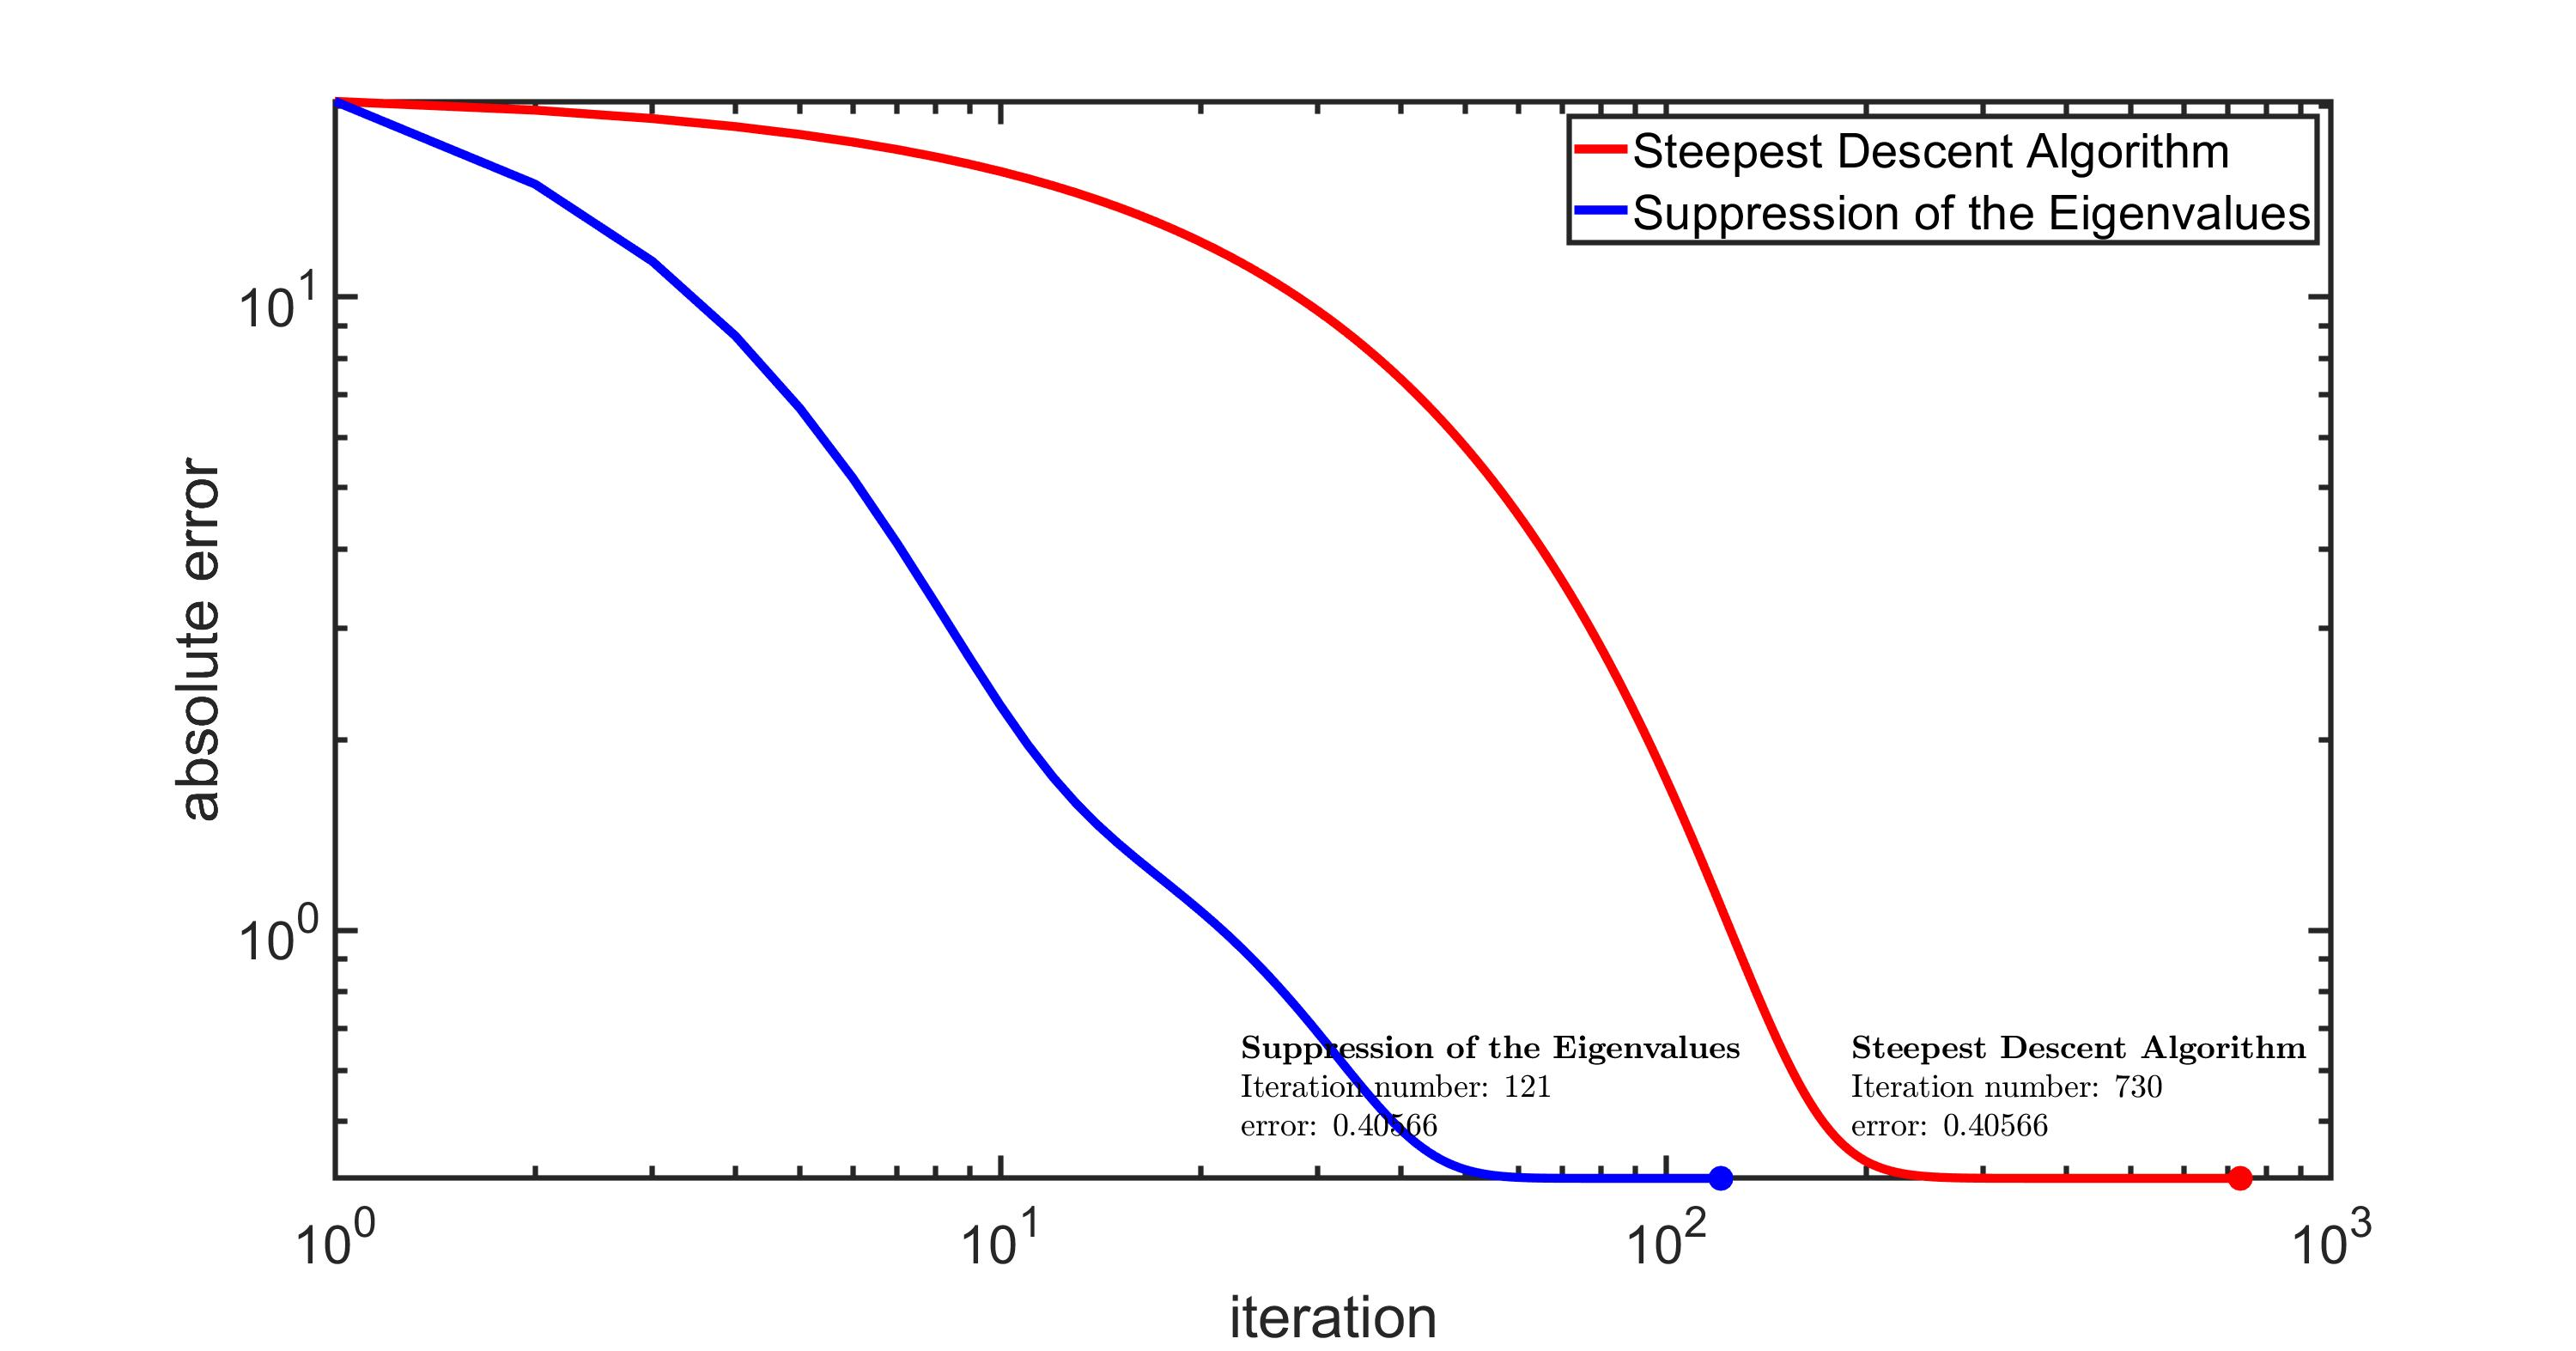
\includegraphics[width=\textwidth]{fig/Ex1_SDAvsSoE.jpg}
		\caption{Error evolution for SDA and SoE for system \eqref{eq:ILC:Sys_ex1}}
		\label{img:ILC:Ex1_SDAvsSoE}
	\end{figure}
	
\end{exam}

\section{Feedback Design}

With the previous algorithms we can achieve a better tracking for repetitively executed processes.  But they do not accent the special features of the model. For example, we can not manage the non-minimum-phase zeros, which can impact the convergence rate \cite{ILC}. 
If we consider the plant structure and construct a feedback controller, and then convert it into a steepest descent-like algorithm, we possibly can achieve better performance and robustness properties. 

Let us denote with $G(z)$ the transfer matrix in variable $z$ of the system $(A,B,C,D)$, and with $G$ the supervector matrix. 

More precisely, we consider a forward path compensator $K_c(z)$ in a unity negative feedback system for \eqref{eq:GP}. 
The design criteria for $K_c(z)$ include the closed-loop stability and the ability to track, albeit approximately, the reference signal $r$. With this compensator, depending on the model, we can remedy the plant properties such as oscillation, loop interaction, or the effects of non-minimum-phase zeros. 

We denote the complementary sensitivity of the resulting closed loop with $T(z)$ and its sensitivity with $S(z)$:
\begin{align}
T(z) = (I + G(z) K_c(z))^{-1}G(z) K_c(z) \text{ and } S(z)  = I - T(z) =  (I + G(z) K_c(z))^{-1}, 
\end{align}

and define the controller
\begin{align}
K_0(z) = K_c(z) S(z). 
\end{align}

Then the compensated Steepest Descent Algorithm is given as follows. 

\begin{alg}
	\label{alg: FBDesign}
	Write the transfer functions in supervector description as 
	$K_0$, $K_c$, $T$ and $S$. The compensated Steepest Descent Algorithm is  is characterized by choosing  $K = \beta K_0$, $\beta \in \R$. 
	The iterative law is given via 
	\begin{align}
	\label{eq:errFBDesign}
	\begin{split}
	u_{k+1} &= u_k + \beta K_0 T^* e_k, \\
	e_{k+1} &= (I- \beta T T^*) e_{k}, \; k\geq 0,\\
	u_0& \in \R^{l (N+1)}. 
	\end{split}	
	\end{align}
	Monotonic convergence to 
	\begin{align}
	\label{eq:FDErrLim} 
	e_\infty  = \lim_{k\to\infty} e_k = P_{\ker[T^*]}e_0,
	\end{align} 
	is guaranteed if
	\begin{align*}
	0 <\beta < \frac{2}{\lama(T T^*)}.
\end{align*}
$T^*$ stays here for conjugate transpose of the matrix $T$. 
\end{alg}
\begin{proof}
	The proof is identical to this in Algorithm \ref{alg:SDA} if consider the system 
	\begin{align}
	\t y = T\t u + \t d.
	\end{align}
\end{proof}

The effect of the operator $T T^*$ can be seen by considering the closed-loop relation 
\begin{align}
y = Tr.
\end{align}
We get a perfect tracking, if $T = I$, which is not achievable by feedback control. Still, we can assume a good tracking if $||T|| \approx 1$. 

Therefore if $K_c$ provides excellent feedback control of $G$, then rapid convergence could be attained with a choice of gain $\beta \approx 1$ \cite{ILC}. % if and the dominant frequency content of the reference $r$ lies in the bandwidth of the closed loop system $T$







